\documentclass{standalone}
\usepackage{tikz}
\usepackage{xcolor}
\usetikzlibrary{patterns, positioning}

    \usetikzlibrary{calc}
    \usepackage{relsize}
    \tikzset{fontscale/.style = {font=\relsize{#1}}}
\begin{document}
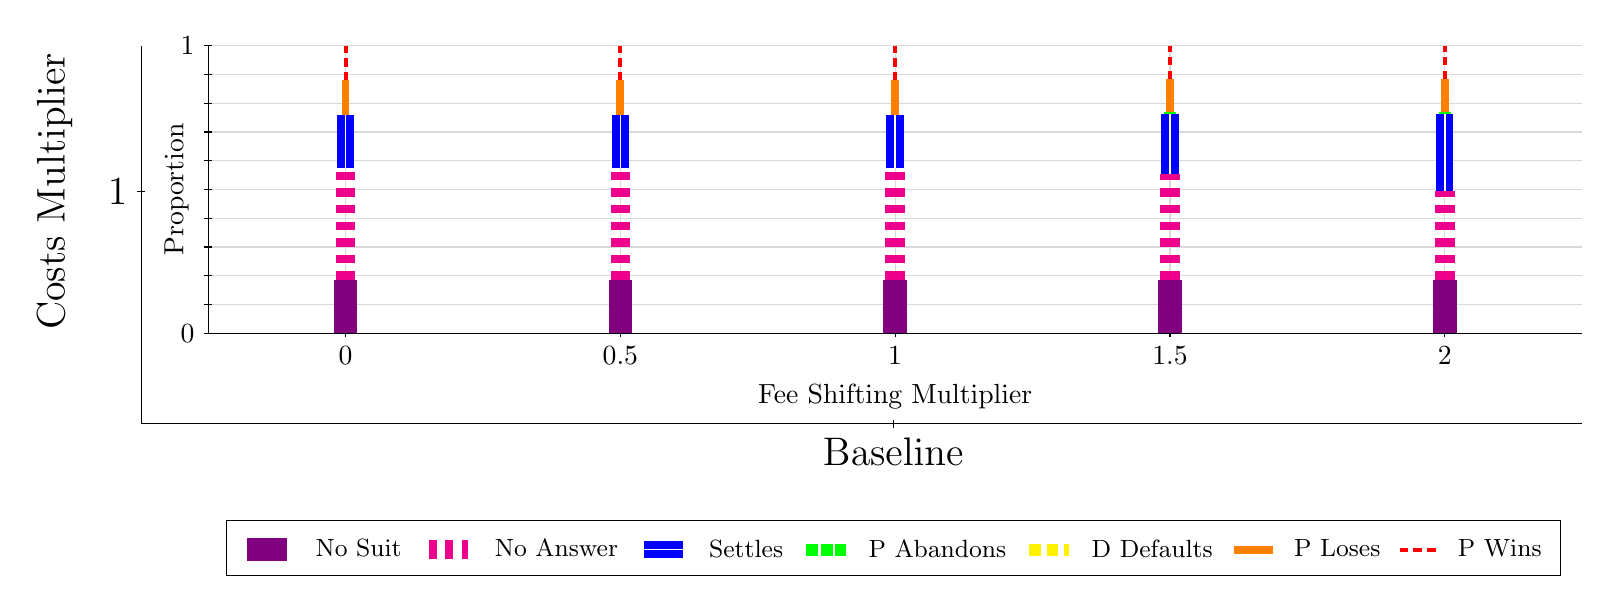
\begin{tikzpicture}
\draw[black] (1.7,1.5) -- (1.7,6.3);
\node[rotate=90, fontscale=2, anchor=center] at (0.6, 4.45) {Costs Multiplier};
\draw[black] (1.65,4.45) -- (1.75,4.45);
\node[fontscale=2, anchor=east] at (1.65, 4.45) {1};

\draw[black] (1.7,1.5) -- (20,1.5);
\node[fontscale=2, anchor=center] at (11.25, 0.6) {};
\draw[black] (11.25,1.45) -- (11.25,1.55);
\node[fontscale=2, anchor=north] at (11.25, 1.45) {Baseline};


\draw[gray!30] (2.55,2.65) -- (20,2.65);
\draw[gray!30] (2.55,3.015) -- (20,3.015);
\draw[gray!30] (2.55,3.38) -- (20,3.38);
\draw[gray!30] (2.55,3.745) -- (20,3.745);
\draw[gray!30] (2.55,4.11) -- (20,4.11);
\draw[gray!30] (2.55,4.475) -- (20,4.475);
\draw[gray!30] (2.55,4.84) -- (20,4.84);
\draw[gray!30] (2.55,5.205) -- (20,5.205);
\draw[gray!30] (2.55,5.57) -- (20,5.57);
\draw[gray!30] (2.55,5.935) -- (20,5.935);
\draw[gray!30] (2.55,6.3) -- (20,6.3);
\draw[gray!30] (4.295,2.65) -- (4.295,6.3);
\draw[gray!30] (7.785,2.65) -- (7.785,6.3);
\draw[gray!30] (11.275,2.65) -- (11.275,6.3);
\draw[gray!30] (14.765,2.65) -- (14.765,6.3);
\draw[gray!30] (18.255,2.65) -- (18.255,6.3);
\draw[black] (2.55,2.65) -- (2.55,6.3);
\node[rotate=90, fontscale=0.7, anchor=center] at (2.15, 4.475) {Proportion};
\draw[black] (2.5,2.65) -- (2.6,2.65);
\node[fontscale=0.7, anchor=east] at (2.5, 2.65) {0};
\draw[black] (2.5,3.015) -- (2.6,3.015);
\node[fontscale=0.7, anchor=east] at (2.5, 3.015) { };
\draw[black] (2.5,3.38) -- (2.6,3.38);
\node[fontscale=0.7, anchor=east] at (2.5, 3.38) { };
\draw[black] (2.5,3.745) -- (2.6,3.745);
\node[fontscale=0.7, anchor=east] at (2.5, 3.745) { };
\draw[black] (2.5,4.11) -- (2.6,4.11);
\node[fontscale=0.7, anchor=east] at (2.5, 4.11) { };
\draw[black] (2.5,4.475) -- (2.6,4.475);
\node[fontscale=0.7, anchor=east] at (2.5, 4.475) { };
\draw[black] (2.5,4.84) -- (2.6,4.84);
\node[fontscale=0.7, anchor=east] at (2.5, 4.84) { };
\draw[black] (2.5,5.205) -- (2.6,5.205);
\node[fontscale=0.7, anchor=east] at (2.5, 5.205) { };
\draw[black] (2.5,5.57) -- (2.6,5.57);
\node[fontscale=0.7, anchor=east] at (2.5, 5.57) { };
\draw[black] (2.5,5.935) -- (2.6,5.935);
\node[fontscale=0.7, anchor=east] at (2.5, 5.935) { };
\draw[black] (2.5,6.3) -- (2.6,6.3);
\node[fontscale=0.7, anchor=east] at (2.5, 6.3) {1};

\draw[black] (2.55,2.65) -- (20,2.65);
\node[fontscale=0.7, anchor=center] at (11.275, 1.85) {Fee Shifting Multiplier};
\draw[black] (4.295,2.6) -- (4.295,2.7);
\node[fontscale=0.7, anchor=north] at (4.295, 2.6) {0};
\draw[black] (7.785,2.6) -- (7.785,2.7);
\node[fontscale=0.7, anchor=north] at (7.785, 2.6) {0.5};
\draw[black] (11.275,2.6) -- (11.275,2.7);
\node[fontscale=0.7, anchor=north] at (11.275, 2.6) {1};
\draw[black] (14.765,2.6) -- (14.765,2.7);
\node[fontscale=0.7, anchor=north] at (14.765, 2.6) {1.5};
\draw[black] (18.255,2.6) -- (18.255,2.7);
\node[fontscale=0.7, anchor=north] at (18.255, 2.6) {2};

\draw[violet, line width=3mm, solid] (4.295,2.65) -- (4.295,3.3292);
\draw[violet, line width=3mm, solid] (7.785,2.65) -- (7.785,3.3292);
\draw[violet, line width=3mm, solid] (11.275,2.65) -- (11.275,3.3292);
\draw[violet, line width=3mm, solid] (14.765,2.65) -- (14.765,3.3292);
\draw[violet, line width=3mm, solid] (18.255,2.65) -- (18.255,3.3292);
\draw[magenta, line width=2.5mm, dashed] (4.295,3.3292) -- (4.295,4.7519);
\draw[magenta, line width=2.5mm, dashed] (7.785,3.3292) -- (7.785,4.7519);
\draw[magenta, line width=2.5mm, dashed] (11.275,3.3292) -- (11.275,4.7519);
\draw[magenta, line width=2.5mm, dashed] (14.765,3.3292) -- (14.765,4.6684);
\draw[magenta, line width=2.5mm, dashed] (18.255,3.3292) -- (18.255,4.4506);
\draw[blue, line width=1mm, double] (4.295,4.7519) -- (4.295,5.4217);
\draw[blue, line width=1mm, double] (7.785,4.7519) -- (7.785,5.4217);
\draw[blue, line width=1mm, double] (11.275,4.7519) -- (11.275,5.4217);
\draw[blue, line width=1mm, double] (14.765,4.6684) -- (14.765,5.44);
\draw[blue, line width=1mm, double] (18.255,4.4506) -- (18.255,5.4304);
\draw[green, line width=1.5mm, densely dotted] (4.295,5.4217) -- (4.295,5.4217);
\draw[green, line width=1.5mm, densely dotted] (7.785,5.4217) -- (7.785,5.4217);
\draw[green, line width=1.5mm, densely dotted] (11.275,5.4217) -- (11.275,5.4217);
\draw[green, line width=1.5mm, densely dotted] (14.765,5.44) -- (14.765,5.4632);
\draw[green, line width=1.5mm, densely dotted] (18.255,5.4304) -- (18.255,5.4632);
\draw[yellow, line width=1.5mm, dotted] (4.295,5.4217) -- (4.295,5.4217);
\draw[yellow, line width=1.5mm, dotted] (7.785,5.4217) -- (7.785,5.4217);
\draw[yellow, line width=1.5mm, dotted] (11.275,5.4217) -- (11.275,5.4217);
\draw[yellow, line width=1.5mm, dotted] (14.765,5.4632) -- (14.765,5.4632);
\draw[yellow, line width=1.5mm, dotted] (18.255,5.4632) -- (18.255,5.4632);
\draw[orange, line width=1mm, solid] (4.295,5.4217) -- (4.295,5.8609);
\draw[orange, line width=1mm, solid] (7.785,5.4217) -- (7.785,5.8609);
\draw[orange, line width=1mm, solid] (11.275,5.4217) -- (11.275,5.8609);
\draw[orange, line width=1mm, solid] (14.765,5.4632) -- (14.765,5.8758);
\draw[orange, line width=1mm, solid] (18.255,5.4632) -- (18.255,5.8758);
\draw[red, line width=0.5mm, densely dashed] (4.295,5.8609) -- (4.295,6.3);
\draw[red, line width=0.5mm, densely dashed] (7.785,5.8609) -- (7.785,6.3);
\draw[red, line width=0.5mm, densely dashed] (11.275,5.8609) -- (11.275,6.3);
\draw[red, line width=0.5mm, densely dashed] (14.765,5.8758) -- (14.765,6.3);
\draw[red, line width=0.5mm, densely dashed] (18.255,5.8758) -- (18.255,6.3);

\draw (11.25,0) node[draw=none] (baseCoordinate) {};
\begin{scope}[align=center]
        \matrix[scale=0.5, draw=black, below=-0.4cm of baseCoordinate, nodes={draw}, column sep=0.1cm]{
        
\draw[violet, line width=3mm, solid] (0.25,-0.25) -- (0.75,-0.25); &
\node[draw=none, font=\small] (B) {No Suit}; &

\draw[magenta, line width=2.5mm, dashed] (0.25,-0.25) -- (0.75,-0.25); &
\node[draw=none, font=\small] (B) {No Answer}; &

\draw[blue, line width=1mm, double] (0.25,-0.25) -- (0.75,-0.25); &
\node[draw=none, font=\small] (B) {Settles}; &

\draw[green, line width=1.5mm, densely dotted] (0.25,-0.25) -- (0.75,-0.25); &
\node[draw=none, font=\small] (B) {P Abandons}; &

\draw[yellow, line width=1.5mm, dotted] (0.25,-0.25) -- (0.75,-0.25); &
\node[draw=none, font=\small] (B) {D Defaults}; &

\draw[orange, line width=1mm, solid] (0.25,-0.25) -- (0.75,-0.25); &
\node[draw=none, font=\small] (B) {P Loses}; &

\draw[red, line width=0.5mm, densely dashed] (0.25,-0.25) -- (0.75,-0.25); &
\node[draw=none, font=\small] (B) {P Wins}; \\
            };
\end{scope}

\end{tikzpicture}
\end{document}